\documentclass[12pt]{article}
\usepackage{times} 			% use Times New Roman font

\usepackage[margin=1in]{geometry}   % sets 1 inch margins on all sides
\usepackage[hidelinks]{hyperref}               % for URL formatting
\usepackage[pdftex]{graphicx}       % So includegraphics will work
\setlength{\parskip}{1em}           % skip 1em between paragraphs
\usepackage{indentfirst}            % indent the first line of each paragraph
\usepackage{datetime}
\usepackage[small, bf]{caption}
\usepackage{listings}               % for code listings
\usepackage{xcolor}                 % for styling code
\usepackage{multirow}
\usepackage{subcaption}     % for subfigures

%\setlength\intextsep{1.69cm} 

%New colors defined below
\definecolor{backcolour}{RGB}{246, 246, 246}   % 0xF6, 0xF6, 0xF6
\definecolor{codegreen}{RGB}{16, 124, 2}       % 0x10, 0x7C, 0x02
\definecolor{codepurple}{RGB}{170, 0, 217}     % 0xAA, 0x00, 0xD9
\definecolor{codered}{RGB}{154, 0, 18}         % 0x9A, 0x00, 0x12

%Code listing style named "gcolabstyle" - matches Google Colab
\lstdefinestyle{gcolabstyle}{
  basicstyle=\ttfamily\small,
  backgroundcolor=\color{backcolour},   
  commentstyle=\itshape\color{codegreen},
  keywordstyle=\color{codepurple},
  stringstyle=\color{codered},
  numberstyle=\ttfamily\footnotesize\color{darkgray}, 
  breakatwhitespace=false,         
  breaklines=true,                 
  captionpos=b,                    
  keepspaces=true,                 
  numbers=left,                    
  numbersep=5pt,                  
  showspaces=false,                
  showstringspaces=false,
  showtabs=false,                  
  tabsize=2
}

\lstset{style=gcolabstyle}      %set gcolabstyle code listing

% to make long URIs break nicely
\makeatletter
\g@addto@macro{\UrlBreaks}{\UrlOrds}
\makeatother

% for fancy page headings
\usepackage{fancyhdr}
\setlength{\headheight}{13.6pt} % to remove fancyhdr warning
\pagestyle{fancy}
\fancyhf{}
\rhead{\small \thepage}
\chead{\small CS 532, Fall 2024} 
\lhead{\small HW\#1, Landers}  % EDIT THIS, REPLACE # with HW number

\setlength{\parindent}{0pt}

%-------------------------------------------------------------------------
\begin{document}

% EDIT THE ITEMS HERE
\begin{centering}
{\large\textbf{HW \#1 - Web Science Intro}}\\ 
Ethan Landers\\
Due: September 15, 2024\\
\end{centering}

%-------------------------------------------------------------------------

% The * after \section just says not to number the sections
\section*{Q1}

Consider the "bow-tie" structure of the web in the Broder et al. paper \textit{"Graph Structure in the Web"} that was described in Module 1.

Now consider the following links:

\begin{verbatim}
A --> B
B --> A
B --> C
C --> D
C --> G
D --> A
D --> H
E --> F
E --> O
F --> G
G --> C
H --> L
J --> N
K --> I
M --> A
N --> L
O --> J    
\end{verbatim}

Draw the resulting directed graph (either sketch on paper or use another tool) showing how the nodes are connected to each other and include an image in your report. This does not need to fit into the bow-tie type diagram but should look more similar to the graph on slide 24 from Module-01 Web-Science-Architecture.

For the graph, list the nodes (in alphabetical order) that are each of the following categories:

\clearpage

\subsection*{Answer}

\begin{figure}[h!]
    \centering
    % trim and clip are used to crop the image, trim=left bottom right top
    % width sets max width, height will be scaled appropriately
    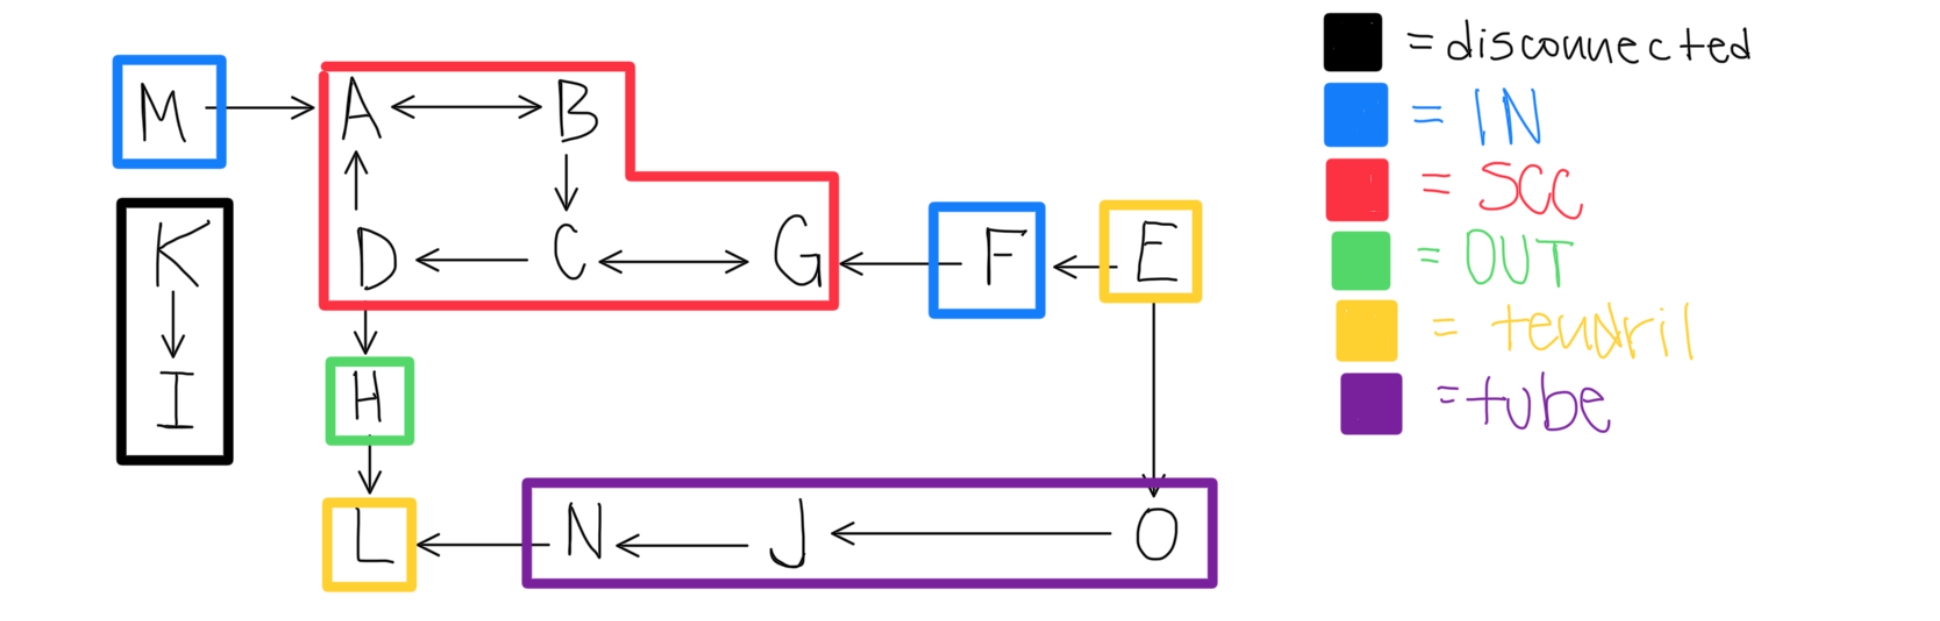
\includegraphics[width=0.8\textwidth] {q1.png}
    \label{fig:directed-graph}
\end{figure}

\begin{itemize}
    \item \textbf{SCC:}
    \begin{itemize}
        \item A
        \item B
        \item C
        \item D
        \item G
    \end{itemize}
    \item \textbf{IN:}
    \begin{itemize}
        \item F
        \item M
    \end{itemize}
    \item \textbf{OUT:}
    \begin{itemize}
        \item H
    \end{itemize}
    \item \textbf{Tendrils:}
    \begin{itemize}
        \item E
        \begin{itemize}
            \item {Node E can reach the IN Node F.}
        \end{itemize}
        \item L
        \begin{itemize}
            \item {Node L can reach the OUT Node L.}
        \end{itemize}
    \end{itemize}
    \item \textbf{Tubes:}
    \begin{itemize}
        \item[] These nodes connect tendril E to tendril L:
        \item J
        \item O
        \item N
    \end{itemize}
    \clearpage
    \item \textbf{Disconnected:}
    \begin{itemize}
        \item I
        \item K
    \end{itemize}
    
\end{itemize}

\section*{Q2}

Demonstrate that you know how to use curl and are familiar with the available options. Complete the following steps using https://www.cs.odu.edu/~mweigle/courses/cs532/ua\_echo.php as the URI to request. Explain the results you get from each step.

\subsection*{Answer}

\begin{enumerate}
    \item First, load the webpage at the URI in your web browser. The result should show the "User-Agent" HTTP request header that your web browser sends to the web server. Take a screenshot to include in your report.
    \begin{figure}[h!]
        \centering
        % trim and clip are used to crop the image, trim=left bottom right top
        % width sets max width, height will be scaled appropriately
        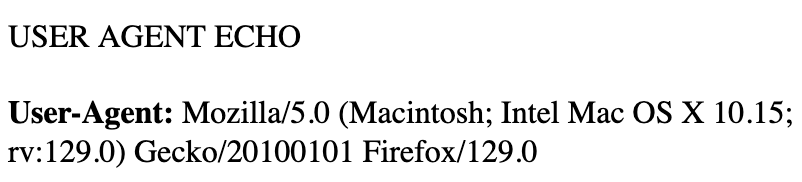
\includegraphics[width=0.8\textwidth] {q2-a.jpg}
        \label{fig:http-request-header}
    \end{figure}

    \item Use a single curl command with the appropriate options to do the following:
    \begin{itemize}
        \item request the URI
        \item show the HTTP response headers
        \item follow any redirects
        \item change the User-Agent HTTP request field to "CS432/532"
        \item[] Take a screenshot of the curl command and options you used and the result of your execution to include in your report.
    \end{itemize}
    \begin{figure}[h!]
        \centering
        % trim and clip are used to crop the image, trim=left bottom right top
        % width sets max width, height will be scaled appropriately
        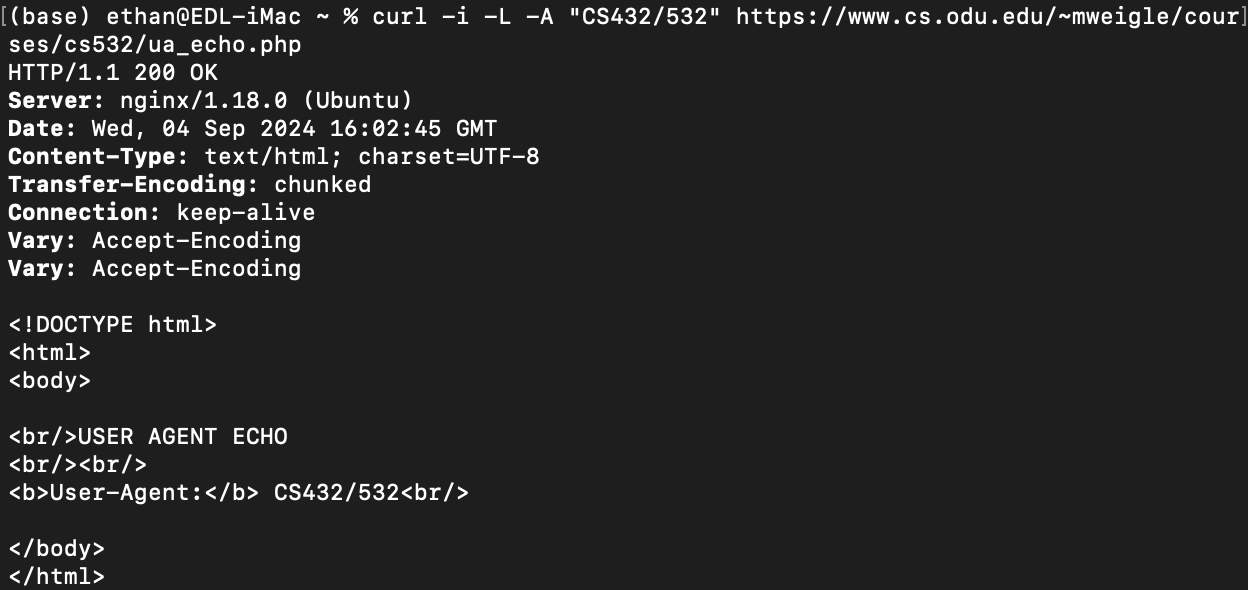
\includegraphics[width=0.8\textwidth] {q2-b.jpg}
        \label{fig:q2-b}
    \end{figure}

    \item Use a single curl command with the appropriate options to do the following:
    \begin{itemize}
        \item request the URI
        \item follow any redirects
        \item change the User-Agent HTTP request field to "CS432/532"
        \item save the HTML output to a file
        \item[] Take a screenshot of the curl command and options you used and the result of your execution to include in your report.
    \end{itemize}
    \begin{figure}[h!]
        \centering
        % width sets max width, height will be scaled appropriately
        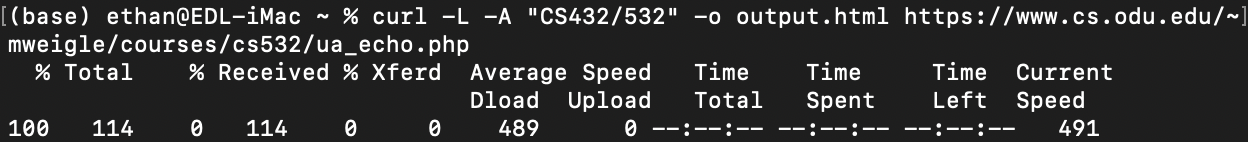
\includegraphics[width=0.8\textwidth] {q2-c.jpg}
        \label{fig:q2-c}
    \end{figure}

    \item View the HTML output file produced by curl from part c in a web browser and take a screenshot to include in your report.
    \begin{figure}[h!]
        \centering
        % width sets max width, height will be scaled appropriately
        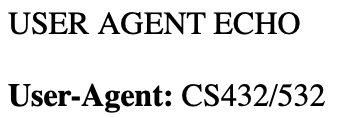
\includegraphics[width=0.8\textwidth] {output.jpg}
        \label{fig:q2-d}
    \end{figure}
    
\end{enumerate}

\clearpage

\section*{Q3}

Your program must do the following:
\begin{enumerate}
    \item take the URI of a seed webpage as a command-line argument
    \item extract all the links from the page's HTML
    \item for each link, request the URI and use the Content-Type HTTP response header to determine if the link references an HTML file (text/html)
    \begin{itemize}
        \item if it does, use the Content-Length HTTP response header to determine if it contains more than 1000 bytes
        \begin{itemize}
            \item if it does, then print the final URI (after any redirects)
        \end{itemize}
    \end{itemize}
\end{enumerate}

Use this program to collect at least 500 unique URIs of web pages that contain more than 1000 bytes. Save the list of URIs to a file to use in later assignments. The file must be uploaded to your GitHub repo.

\subsection*{Answer}
\begin{enumerate}
    \item I created a check to ensure that the user provided a command-line seed URI argument when running the program:
    \begin{lstlisting}[language=Python, label=lst:copy]
    if __name__ == "__main__":
    # Ensure the user provided a command-line argument
    if len(sys.argv) != 2:
        print("Usage: python3 collect-webpages.py <seed_uri>")
        sys.exit(1)

    # Start the main process with the provided seed URI
    main(sys.argv[1])
    \end{lstlisting}
    If the user doesn't provide a command-line argument, a message will appear directing the user to the correct way to run the program, which would include a command-line argument.

    \item I created a function to extract all links from a given webpage:
    \begin{lstlisting}[language=Python, label=1st:copy]
def extract_links_from_page(uri):
    print(f"Fetching page: {uri}")
    try:
        response = requests.get(uri, timeout=5, verify=False)
        
        # Parse the HTMl content using BeautifulSoup
        soup = BeautifulSoup(response.text, 'html.parser')
        links = set()
        
        for link in soup.find_all('a', attrs={'href': re.compile("^https://")}):
            href = link.get('href')
            if href:
                links.add(href)

        print(f"Found {len(links)} links on page")
        return links
    
    except requests.exceptions.RequestException as e:
        print(f"Error fetching {uri}: {e}")
        return set() # Return an empty set if there is an error
    \end{lstlisting}
    The requests library makes HTTP GET requests to the provided URI. BeautifulSoup parses HTML pages and extracts links that start with HTTP://. The links are then returned as a set to ensure uniqueness. The code includes a few debug statements.

    \item I created a function to verify if links are valid HTML pages:
     \begin{lstlisting}[language=Python, label=1st:copy]
def is_valid_html_page(uri):
    print(f"Validating URI: {uri}")
    try:
        response = requests.head(uri, timeout=5, verify=False)
        content_type = response.headers.get('Content-Type', '')
        content_length = response.headers.get('Content-Length', 0)

        if 'text/html' in content_type and int(content_length) > 1000:
            print(f"Valid HTML page: {uri}")
            return True
        else:
            print(f"Invalid HTML page or too small: {uri}")
            return False
    
    except requests.exceptions.Timeout as e:
        print(f"Timeout error validating {uri}: {e}")
        return False
    except requests.exceptions.RequestException as e:
        print(f"Error validating {uri}: {e}")
        return False
     \end{lstlisting}
    This function returns boolean variables by checking HTML headers to determine whether they are valid HTML pages and whether they have more than 1000 bytes. Exception states are printed otherwise.

    After the HTML pages are verified, they will be added to a set of URIs and printed to an output file called uris.txt.  
     
\end{enumerate}

The program randomly picks a URI from the provided seed URI and uses that as the new seed until 500 unique URIs are collected.

Here is a screenshot of what a part of the currently generated output file uris.txt looks like when the seed URI \url{https://weiglemc.github.io/} is used:
\begin{figure}[h!]
    \centering
    % width sets max width, height will be scaled appropriately
    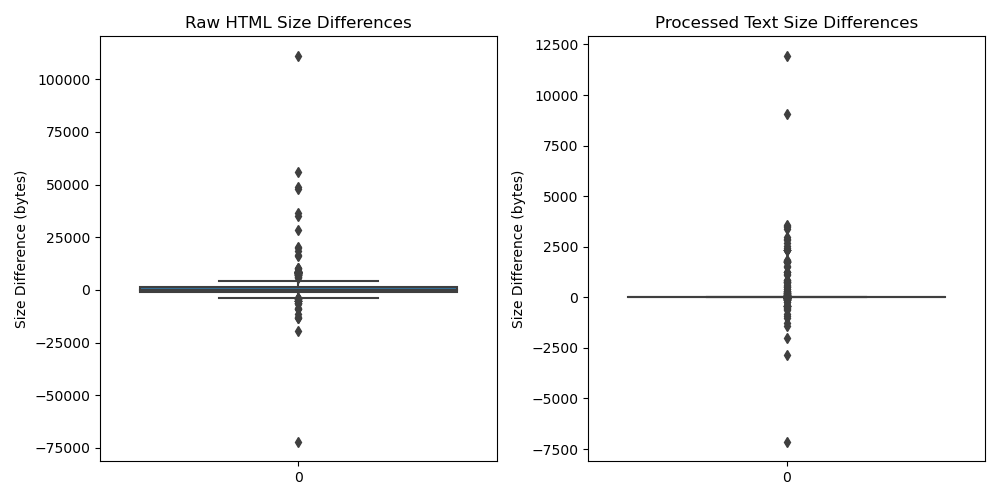
\includegraphics[width=0.8\textwidth] {q3.png}
    \label{fig:q3}
\end{figure}

\section*{References}

\begin{itemize}
    \item {Overleaf documentation, \url{https://www.overleaf.com/learn}}
    \item {Curl documentation, \url{https://curl.se/docs/manpage.html}}
    \item {Python Virtual Environments, \url{https://python.land/virtual-environments/virtualenv}}
    \item{Python Data Types, \url{https://www.geeksforgeeks.org/python-data-types/}}
    \item{Implementing Web Scraping with BeautifulSoup, \url{https://www.geeksforgeeks.org/implementing-web-scraping-python-beautiful-soup/}}
    \item{BeautifulSoup Scraping Link from HTML, \url{https://www.geeksforgeeks.org/beautifulsoup-scraping-link-from-html/?ref=header_outind}}
    \item{Exception Handling in Python Requests Module, \url{https://www.geeksforgeeks.org/exception-handling-of-python-requests-module/}}
    \item{Python Random Choice Method, \url{https://www.w3schools.com/python/ref_random_choice.asp}}
    \item{Writing to File in Python, \url{https://www.geeksforgeeks.org/writing-to-file-in-python/}}
\end{itemize}

\end{document}

